\documentclass[a4paper]{paper}

% Set margins
\usepackage[hmargin=2cm, vmargin=2cm]{geometry}

\frenchspacing

% Language packages
\usepackage[utf8]{inputenc}
\usepackage[T1]{fontenc}
\usepackage[magyar]{babel}

% AMS
\usepackage{amssymb,amsmath}

% Graphic packages
\usepackage{graphicx}

% Colors
\usepackage{color}
\usepackage[usenames,dvipsnames]{xcolor}

% Enumeration
\usepackage{enumitem}

\begin{document}

\begin{center}
    \Large
    \textbf{Négykerekű járművek navigációs problémáinak megoldása}

    \medskip   

    \Large
    Tóth Péter
\end{center}

\vskip 1cm

\pagestyle{empty}

\section{A megoldandó probléma}

Négykerekű járművek navigálási problémáinak részletes leírása. Feltételezzük, hogy a térkép felülnézetből ismert. Az optimalizálás célja azon navigációs műveleteknek a meghatározása, amely segítségével a jármű adott pozícióból a térkép járható területein keresztül el tud jutni a célként megadott pozícióba. Fel kell írni az optimalizálási feladatokat különböző célfüggvények figyelembevételével. Meg kell jeleníteni az algoritmus által adott útvonalakat. Az optimalizálási probléma megoldása Python programozási nyelven történik a NumPy függvénykönyvtár felhasználásával.

\section{Kétkerekű modell kanyarodási íve}

A kétkerekű (bicikli) modell kanyarodási ívének meghatározása 2 dologtól függ:\newline
\phantom{asd} - a tengelytávolságtól (w),\newline
\phantom{asd} - az első kerék kanyarodási szögétől ($\alpha$).\newline
Az első és hátsó kerekek is egy-egy körpályát fognak követni azonos középponttal. Az irány mindig merőleges a sugárra.

\begin{figure}[h!]
\centering
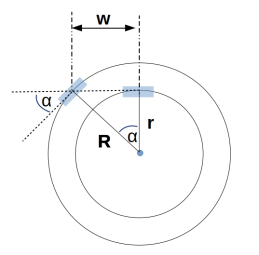
\includegraphics[scale=0.5]{images/two_wheels_rad.png}
\caption{Kétkerekű jármű kanyarodási íve}
\label{fig:two_wheels_rad}
\end{figure}

Az ábrán R az első kerékhez tartozó sugár, r pedig a hátsó kerékhez.\newline
Az első kerék pályája: $\sin\alpha$ = $\cfrac{w}{R}$ \hspace{5mm}---> \hspace{5mm} $R$ = $\cfrac{w}{\sin\alpha}$ \newline
A hátsó kerék pályája: $\tan\alpha$ = $\cfrac{w}{r}$ \hspace{5mm}---> \hspace{5mm} $r$ = $\cfrac{w}{\tan\alpha}$
\newpage

\section{A jármű matematikai modellje}

A négykerekű jármű középpontjának a hátsó tengely középpontját tekintjük. Mivel a kanyarodásnál az első kerekek különböző szögeket zárnak be az első tengellyel, ezért érdemes egy képzeletbeli, az első tengely közepére eső kormányozható kereket megadni. Ennek a jármű irányával bezárt előjeles szögét jelöljük $\alpha$-val. A jármű tengelytávolságát jelöljük $w$-vel, a hátsó tengely hosszát pedig $a$-val (\ref{fig:vehicle}. ábra).

\begin{figure}[h!]
\centering
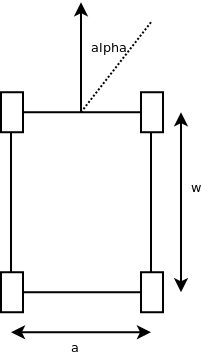
\includegraphics[scale=0.45]{images/vehicle.png}
\caption{A jármű matematikai modelljének fő paraméterei}
\label{fig:vehicle}
\end{figure}

\section{Első kerekek elfordulási szögének kiszámítása}

Az $\alpha$ szög függvényében külön ki kell számítanunk a jármű bal és jobb első kerekének elfordulási szögét.
Tehát első lépésben határozzuk meg az adott $\alpha$ szög ismeretében a további számításokhoz szükséges sugarat,
melyet a \ref{fig:turning_vehicle}. ábrán R jelöl. Ez a kanyarodási sugár, melyet a jármű középvonalához mérünk. Az ehhez szükséges képlet:\vspace{2mm}
$R$ = $\dfrac{w}{\text{tg} \alpha}$ \vspace{5mm}

Továbbiakban a jelölések ugyanazok, az első kerekeket tekintve pedig $\alpha\textsubscript{1}$ a belső, $\alpha\textsubscript{2}$ pedig a külső kerék elfordulási szögét jelöli. 
A jármű tengelytávolsága, valamint szélessége, és a sugár ismeretében ezen két szög a következőképpen számítható ki:\newline\
$\alpha\textsubscript{1}$ = $\text{arctan}\Bigg(\cfrac{w}{R-\frac{a}{2}}\Bigg)$ \hspace{1cm} $\alpha\textsubscript{2}$ = $\text{arctan}\Bigg(\cfrac{w}{R+\frac{a}{2}}\Bigg)$


\begin{figure}[h!]
\centering
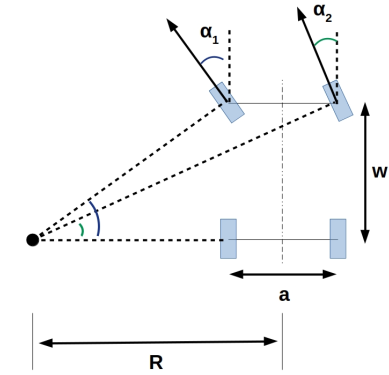
\includegraphics[scale=0.5]{images/turning_vehicle.png}
\caption{Első kerekek elfordulási szögei}
\label{fig:turning_vehicle}
\end{figure}


% TODO: Részletesen leírni ezek számítását!

\section{Pozíció számítása rögzített $\alpha$ mellett}

A rögzített $\alpha$ szög, és adott sebesség mellett ki kell tudnunk számolni, hogy adott $(x_0, y_0)$ kiindulópontból indulva a jármű milyen pozícióba fog kerülni $t$ idő elteltével. Az $\alpha$ szög függvényében az alábbi módon számolhatjuk ki annak a képzeletbeli körnek a sugarát ($R$), amelyen a jármű majd kanyarodni fog:
\[
R = \dfrac{w}{\text{tg} \alpha},
\]
ahol a $w$ a jármű tengelyei közötti távolságot jelöli.

Tegyük fel, hogy a jármű sebessége $v$. Ekkor $t$ idő függvényében a jármű pozícióját az alábbi formában számolhatjuk:
\begin{align*}
x(t) &= x_0 + R - R \cdot \cos \dfrac{v \cdot t}{|R|}, \\
y(t) &= y_0 + |R| \cdot \sin \dfrac{v \cdot t}{|R|}.
\end{align*}

\section{Útvonal meghatározása az eltelt idő függvényében}

$$
\vec{v} \in \mathbb{R} \hspace{0.5cm}
\quad \rightarrow \quad
\vec{v} (t) \colon \mathbb{R} \to \mathbb{R}^2
$$

Elfordulás:
$$
\varphi (t) \hspace{0.5cm} \rightarrow \hspace{0.5cm} \vec{v} (t) =
\begin{bmatrix}
\cos(\varphi(t)) \\
\sin(\varphi(t))
\end{bmatrix}
$$

$ \vec{x_0} $ : kezdőpozíció

Egy egységnyi idő elteltével az irány: $ \vec{x} (t_1) = \vec{x_0} + \displaystyle\int_{t_0}^{t_1} \vec{v} (t) dt $

Általános alak:  $ \vec{x} (t) = \vec{x_0} + \displaystyle\int_{t_0}^{t} \vec{v} (u) du $

$$
\begin{bmatrix} x_1 \\ y_1 \end{bmatrix} = \begin{bmatrix} x_0 \\ y_0 \end{bmatrix} + \displaystyle\int_{t_0}^{t_1} \begin{bmatrix} \cos(\varphi(t)) \\ \sin(\varphi(t)) \end{bmatrix} dt
$$

Külön a két vektort leintegráljuk:

\begin{align*}
x_1 &= x_0 + \displaystyle\int_{t_0}^{t_1} \cos(\varphi(t)) \; \mathrm{d}t \\
y_1 &= y_0 + \displaystyle\int_{t_0}^{t_1} \sin(\varphi(t)) \; \mathrm{d}t \\
\end{align*}

\end{document}
